\documentclass[12pt]{article}

\input{setup}

% \addbibresource{tnd.bib}

\begin{document}
%TC:ignore
\begin{titlepage}
\title{Inferring infectiousness: a joint model of the within-host viral kinetics of SARS-CoV-2}
\author[1]{Christopher Boyer\thanks{email: \href{mailto:cboyer@hsph.harvard.edu}{cboyer@hsph.harvard.edu}}}
\author[1,2]{Marc Lipsitch}
\affil[1]{Department of Epidemiology, Harvard T.H. Chan School of Public Health, Boston, MA.}
\affil[2]{Department of Immunology and Infectious Diseases, Harvard T.H. Chan School of Public Health, Boston, MA.}
\date{\today}
\maketitle

\begin{abstract}
During an infectious disease outbreak, providing accurate answers to many policy questions about transmission requires a detailed model of the natural history of infectiousness. Unfortunately, direct measures of infectiousness are generally unavailable. Instead, we often rely on proxies of within-host viral kinetics such as symptoms or results from antigen and PCR tests or viral culture. However, these proxies vary in terms of the ease of collection, scalability, and their relationship to viral shedding and therefore underlying infectiousness. Here, we use data from four prospective, densely sampled cohorts with longitudinal data on multiple proxies of viral shedding for approximately 2,000 infections to develop a Bayesian joint model for the within-host viral kinetics of SARS-CoV-2 infection. Modeling the joint distribution allows us to infer the possible values of harder to measure proxies at any point during the infection based on all the available data. 
\noindent \\
\vspace{0in} \\
\noindent\textit{Keywords:} 
\bigskip
\end{abstract}
\setcounter{page}{0}
\thispagestyle{empty}
\end{titlepage}
\pagebreak \newpage
\spacingset{1.45} % DON'T change the spacing!
%\setstretch{1.5}
\section{Introduction} \label{sec:introduction}
Accurate information about the internal dynamics of infection within a host are crucial for informing effective public health policies during outbreaks. Chief among these are the infectious period \textemdash the period of time in which a host is able to transmit infection to another individual---  and an individual's infectiousness \textemdash the current probability of onward transmission given contact with another susceptible host. Both parameters are essential for shaping policy recommendations on managing illness and are also critical inputs for building accurate transmission models. However, direct measurement of infectiousness poses significant challenges. As a result, researchers often rely on proxies of viral shedding, such as self-reported symptoms, antigen and polymerase chain reaction (PCR) test results, or viral culture data, to estimate infectiousness.

These proxies vary widely in their ease of collection, scalability, and correlation with actual viral shedding. Symptom-based assessments are subjective and can be influenced by individual variability and reporting biases. Antigen tests offer rapid results but may lack sensitivity, especially in asymptomatic individuals or at different stages of infection. PCR tests are highly sensitive but can detect non-viable viral RNA, potentially overestimating the period of infectiousness. Viral culture is considered the gold standard for assessing infectivity but is labor-intensive and not feasible for large-scale or rapid assessments.

The reliance on single proxies or sparsely collected data can lead to incomplete or inaccurate representations of an individual's infectiousness over time. This limitation hampers our ability to answer critical policy questions, such as determining optimal isolation periods or prioritizing testing strategies. There is a clear need for a comprehensive approach that integrates multiple proxies to more accurately model within-host viral kinetics.

In this study, we address this gap by developing a Bayesian joint model for the within-host viral kinetics of SARS-CoV-2 infection. Utilizing data from four prospective, densely sampled cohorts comprising approximately 2,000 infections, we integrate longitudinal measurements of multiple proxies of viral shedding. The Bayesian framework allows us to account for the uncertainties inherent in each proxy and to model their joint distribution over the course of infection.

By modeling the joint distribution, we can infer the likely values of harder-to-measure proxies at any given point during the infection based on the available data. This approach enhances the granularity and accuracy of the viral kinetics profiles, providing a more detailed understanding of infectiousness dynamics. It also facilitates the estimation of unobserved or missing data points, which is particularly valuable in real-world settings where complete data collection is often impractical.

Our findings have significant implications for public health policy and infectious disease modeling. A more accurate representation of within-host viral kinetics can improve transmission models, leading to better-informed decisions regarding intervention strategies such as quarantine durations, contact tracing, and resource allocation. Furthermore, the methodological framework we present is adaptable and can be applied to other infectious diseases, enhancing its utility beyond SARS-CoV-2.

In the sections that follow, we detail the methods used to develop our Bayesian joint model, present the results of our analyses, and discuss the implications of our findings for both modeling efforts and public health policy. By integrating multiple proxies of viral shedding, we aim to provide a robust tool for improving our understanding of infectiousness and enhancing the effectiveness of outbreak response strategies.



\section{Proxies for infectiousness} \label{sec:proxies}
The transmission of a viral pathogen between humans is a complex biological process influenced not only by within-host dynamics of infection but also by a variety of other environmental and behavioral factors. Consequently, measurement and quantification of infectiousness is challenging as it is contingent upon multiple forces. Nonetheless, a key component of infectiousness is the amount of replication competent virus shed by an infected individual, which is more easily observable. Therefore, we focus on modeling viral shedding and assume it is largely synonymous with individual infectiousness, although our model could, in principle, be extended to include additional environmental and behavioral determinants of transmission.

There are several approaches to measuring or inferring viral shedding that vary in terms of their accuracy, ease of use,cost, and scalability. We review the most common below.

\subsection{Infectious virus}
%A necessary pre-requisite for onward transmission of viral infection is the presence of infectious (that is, replication competent) virus. 
The gold standard diagnostic approach to determining whether replication competent virus is present is recovery via cell culture. This is achieved by innoculating susceptible cell lines with clinical specimen and measuring cytopathic effects via light microscopy, with infection confirmed either via RT-PCR of the supernatant of infected cells or by immunostaining for viral proteins. In the case of SARS-CoV-2, several cell lines can be used for isolation including a line from African green monkey kidney cells (Vero E6) and human lines from colorectal adenocarcinoma cells (Caco-2), lung adenocarcinoma cells (A549), and hepatocellular carcinoma cells (Huh7). These lines typically express either angiotensin converting enzyme 2 (ACE2; the receptor required for virus entry) or transmembrane protease 2 (TMPRSS2; another receptor important for virus entry).

While simple culture provides a qualitative assessment of the presence of infectious virus in an innoculated specimen, other methods are available that directly quantify the number of infectious virions. To produce viral titres, the specimen is serially diluted and used for innoculation. In a focus-forming assay, a monolayer of cells is innoculated with the clinical specimen and the cells are fixed one day after infection and immunostained with virus-specific antibodies creating visible groups of infected cells (foci) that can be counted. In a plaque-forming assay, a monolayer of cells is innoculated and plates are fixed 2-3 days post-infection and then stained with crystal violet, forming plaques in the presence of infectious virus that can be counted. Finally, in a 
50\% tissue culture infectious dose (TCID$_{50}$), a monolayer is innoculated and at 

The advantages of viral culture assays are that they directly detect replication competent virus and therefore come the closest to measuring infectious viral shedding. The disadvantages are that cultures are time-consuming and require specially trained laboratory personnel to properly handle and store. Results can vary substantially across cell lines or laboratories. In the case of an emerging pathogen like SARS-CoV-2, cultures had to be performed under biosafety level 3 laboratory conditions. For these reasons, cultures are often expensive and not routinely performed in the clinical setting. Therefore high quality cultures collected longitudinally within the same infection are rare.

\subsection{Viral nucleic acids}
In the clinical setting, laboratory diagnosis of viral infection generally relies instead on demonstration of viral RNA via a virus-specific RT-PCR performed on the clinical specimen. The amount of viral RNA in the sample can be quantified by calibrating the cycle threshold (Ct) value, representing the number of amplification cycles necessary to detect a signal, to reference samples containing proscribed number of viral copies per milliliter or swab. Following previous literature, we refer to this measure of viral RNA concentration as viral load. The strong correlation between viral load and infectious virus leads to its utility as proxy for infectiousness.

RT-PCR is highly sensitive and specific, and thus the gold standard for clinical diagnosis, but it does not distinguish between replication competent and residual RNA. For determining individual infectiousness, this creates challenges particularly in the late stages of infection when destroyed or inactivated virus creates a surfeit of residual RNA leading to positive results even when virions are not themselves infectious. Unlike viral culture RT-PCR assays can be standardized and scaled for mass testing in laboratory settings. They are therefore more commonly used in research, including in longitudinal studies. However, outside certain mass testing, quarantining, or occupational health environments, repeated testing with RT-PCR in the community, as a means for individuals to monitor infectiousness, is not available.

\subsection{Viral antigens}
Diagnostics that can be used in a household or community setting are more restricted. However, since the COVID-19 pandemic, there has been a surge in availability of antigen-detecting rapid diagnostic tests. These tests detect viral proteins from lysed samples by forcing them across a lateral flow field containing conjugate antibody, hereafter referred to as a lateral flow device (LFD). For SARS-CoV-2 tests, the nucleocapsid proteins are typical target antigens of LFDs. In their basic form, LFDs provide a qualitative assessment of whether viral antigen is present but there is often no set procedure for quantifying the amount or concentration, although some studies have attempted to develop grading systems based on the intensity of the test line and a handful of companies offer digital lateral flow reader that provide quantitative results. 

The advantages of LFDs are their speed and simplicity, allowing them to be used at home for more biologically-informed and individualized screening and isolation decisions. Although they can be inaccurate relative to RT-PCR when used for clinical diagnosis, LFDs do correlate strongly with the presence of infectious virus. LFD results can vary by manufacturer, whether they were self-swabbed or taken by a professional, and the type of sample (nasal versus oral). There has also been considerable interest in whether performance may vary across variants. 

\subsection{Symptoms}
Symptom-based assessment is the oldest and most widely accessible approach to inferring infectiousness. Common symptoms of acute respiratory viral infections include cough, sore throat, congestion, fever, fatigue, and myalgia. These symptoms are broadly understood to reflect the host innate and adaptive immune response to infection rather than direct viral cytopathology, which is why symptom onset typically lags behind the initial rise in viral shedding by one to several days. The temporal relationship between viral kinetics and symptom onset is of direct public health relevance: if symptoms reliably coincide with or precede peak infectiousness, symptom-based isolation may be an effective strategy for reducing onward transmission. However, if symptoms substantially lag or fail to appear, as in asymptomatic or pre-symptomatic infections, symptom-based strategies will miss a considerable proportion of infectious person-time.

The advantages of symptom-based assessments are their simplicity and universality --- they require no laboratory infrastructure and can be self-reported. For these reasons, symptom-based screening and isolation policies have been the backbone of pandemic response since well before the availability of modern diagnostics. The disadvantages are substantial. Symptom presentation is subjective and varies considerably across individuals, with some infections remaining entirely asymptomatic. For SARS-CoV-2, estimates of the asymptomatic fraction have ranged from 20\% to over 40\%, and even among symptomatic individuals the time from infection to symptom onset is variable. Furthermore, symptom diaries are subject to reporting biases, recall error, and inconsistent definitions across studies. Despite these limitations, the temporal relationship between symptoms and viral shedding contains information about the immune response that is not captured by virological proxies alone, motivating its inclusion as a component of a joint model.

\section{The model} \label{sec:model}
We propose a generative model of within-host viral kinetics during an acute infection that can be linked, through an observational process, to multiple measures of viral shedding. Consider longitudinal observations from $i = 1, \ldots, N$ infected individuals at times $t = 1, \ldots, T$ since innoculation. The data are realizations $\{(V_{it}, R_{it}, Y_{it}, \mathbf{Z}_{it}, \mathbf{X}_i, S_{i})\}$ where $V_{it}$ is infectious virus, $R_{it}$ is viral RNA copies, $Y_{it}$ is an indicator of symptom onset, $\mathbf{Z}_{it}$ is a vector of observed test or biomarker measurements, $\mathbf{X}_i$ is a vector of individual covariates (e.g. sex, age, immune history), and $\mathbf{S}_i$ is a vector of test characteristics, such as swab type and gene target. The vector $\mathbf{Z}_{it}$ contains proxy measurements for viral shedding including as viral culture ($V^*_{it}$), RT-PCR ($R^*_{it}$), and lateral flow tests for viral antigens ($L^*_{it}$), such that $\mathbf{Z}_{it} = (V^*_{it}, R^*_{it}, L^*_{it})$. We use the superscript $*$ to denote observed rather than true value and, for notational convenience, hereafter we suppress the indexes $i$ for individuals. 

Our goal is to characterize the joint distribution, 
$$
f(V_t, R_t, Y_t, \mathbf{Z}_t | \mathbf{X}, t, S; \theta)
$$
defining the within-host trajectories of viral shedding and test or biomarker results over time, where $\theta$ is a vector of parameters (we use $\theta$ generically throughout to represent as yet to be defined model parameters). To specify the model, we factorize the joint distribution into a product of conditional distributions. A natural factorization is:
\begin{align*}
    f(&V_t, R_t, Y_t, \mathbf{Z}_t | \mathbf{X}, S, t; \theta) = \\ & \quad \underbrace{f(V_t | \mathbf{X}, t; \theta)}_{\shortstack{infectious \\ virus}} \times \underbrace{f(R_t | V_t, \mathbf{X}, t; \theta)}_{\shortstack{viral RNA}} \times \underbrace{f(Y_t | V_t, R_t, \mathbf{X}, t; \theta)}_{\shortstack{natural history \\ of symptoms}} \times \underbrace{f(\mathbf{Z}_t | V_t, R_t, Y_t, \mathbf{X}, t, S; \theta)}_{\shortstack{observation \\ model}}
\end{align*}
where the first term describes the trajectory of infectious virus over time, the second term describes the total concentration of viral RNA over time conditional on the amount of infectious virus, the third term describes the onset of symptoms conditional on the amount of infectious virus and viral RNA, and the fourth term relates these to observed biomarker values and test results.

We posit models for each of these components in turn below.

\subsection{Infectious virus}
A commonly used mechanistic model describing the dynamics of viral proliferation during acute infection is the target cell limited model. In its simplest form, the model tracks the number of susceptible cells ($T$), infected cells ($I$), and free virions ($V$), described by the following system of ordinary differential equations:
\begin{align*}
    \dfrac{dT}{dt}&= -b V T \\
    \dfrac{dI}{dt}&= b V T - d I \\
    \dfrac{dV}{dt}&= p I - c V
\end{align*}
Target cells become infected at rate $b$ upon contact with free virus. Infected cells produce virus at rate $p$ and die at per capita rate $d$, while free virus is cleared at rate $c$. Extensions of this model include the addition of an eclipse phase, in which infected cells do not yet produce virus, and the inclusion of the immune response. An example numerical solution for the trajectory of viral particles over time is shown in Figure X. We note the following salient features: an initial exponential expansion of the infected cell population and number of free virus particles (proliferation), followed by a peak and subsequent exponential decline due to immune response and depletion of susceptible target cells (clearance).

Due to the complexity of the human immune response and the challenges of measuring the initial number of target or infected cells, it is often difficult to specify the target cell model in practice. Therefore, we instead posit a semi-mechanistic model which retains many of the phenomenological features of the model, but is agnostic to the true biological structure of the response. Namely, we assume that the number of infectious viral particles follows a piece-wise exponential function, defined as
\begin{equation*}
    \log V_t = g(t; \theta),
\end{equation*}
where
\begin{equation*}
    g(t; \theta) = \begin{cases}
   \dfrac{\delta}{\omega_p} (t - (t_p - \omega_p)) & \text{if } t \leq t_p \\
    \delta - \dfrac{\delta}{\omega_r} (t - t_p) & \text{if } t > t_p,
\end{cases}
\end{equation*}
with parameters representing peak number of infectious virus ($\delta$), proliferation time ($\omega_p$), clearance time ($\omega_r$), and time of peak ($t_p$), all of which can potentially vary with covariates $\mathbf{X}$. The dotted line in Figure X shows an example trajectory of the number of infectious viral particles over time super-imposed on the numerical solution from the target cell limited model. A notable limitation is that the piece-wise exponential model tends to overestimate the peak value (in our experience by between X and Y\%). However, for our purposes it is a useful approximation which is easier to fit and directly parameterizes many of the quantities of interest, such as the time to peak and the time to clearance.

\paragraph{Smooth trajectory approximation.} The piecewise exponential function has a non-differentiable kink at the peak, which can create challenges for gradient-based sampling. We therefore also consider a smooth approximation based on the log-sum-exp envelope of the two exponential arms. Defining the proliferation rate $a = \delta / \omega_p$ and the clearance rate $b = \delta / \omega_r$, the smooth trajectory is
\begin{equation*}
    g_s(t; \theta) = \delta + \log \frac{a + b}{b \exp(-a(t - t_p)) + a \exp(b(t - (t_p + \omega_f)))}
\end{equation*}
where $\omega_f \geq 0$ is a \emph{flat-top duration} parameter that introduces an approximate plateau of width $\omega_f$ days around the peak. When $\omega_f = 0$, the function reduces to the standard smooth two-arm envelope and collapses to the piecewise exponential in the limit. For $\omega_f > 0$, the rising and falling arms are separated by $\omega_f$ days, approximating a flat peak. To prevent the log-sum-exp envelope from overshooting $\delta$ when $\omega_f > 0$ (an inherent artifact of merging two separated exponential arms), we apply a soft cap:
\begin{equation*}
    \tilde{g}_s(t; \theta) = g_s(t; \theta) - \frac{1}{\kappa}\log\!\left(1 + \exp\!\left(\kappa \left(g_s(t; \theta) - \delta\right)\right)\right)
\end{equation*}
where $\kappa = 10$ controls the sharpness of the cap. This ensures $\tilde{g}_s \leq \delta$ everywhere while maintaining smooth gradients. The resulting trajectory is continuously differentiable, which improves the efficiency of Hamiltonian Monte Carlo sampling.

\subsection{Viral RNA copies}
Many tests, such as RT-PCR, detect or quantify viral RNA rather than infectious virus. That is, they do not distinguish between replication-competent (infectious) virus and residual (non-infectious) viral RNA which could be present due to production of nonviable viral particles during infection or may linger in a nonviable but not fully degraded state after the infection has been cleared by the immune system. In the target cell limited model, we could track the amount of viral RNA via additional compartments. For instance, we could add compartments tracking the number of  free floating RNA ($R$) via 
\begin{equation*}
    \dfrac{dR}{dt} = q p I - e R 
\end{equation*} 
where $q$ the amount of viral RNA per infectious virion and $e$ is the rate of degradation and clearance of viral RNA. However, we do not have direct measurements of the number of viral RNA copies, and the relationship between the number of infectious virus and the number of viral RNA copies is not well understood. Therefore, we again posit a semi-mechanistic model for the number of viral RNA copies. We assume that the number of RNA copies follows the same functional form as the infectious virus trajectory (piecewise or smooth, as described above), with a shared flat-top duration $\omega_f$:
\begin{equation*}
    \log R_t = g(t; \theta^\prime),
\end{equation*}
where $g$ is either the piecewise or smooth function and the RNA-specific parameters $\theta' = (\delta^\prime, \omega^\prime_p, \omega^\prime_r, t^\prime_p, \omega_f)$ are derived from the PFU parameters via
\begin{align*}
    \log \delta^\prime &= a_{0,\delta} + a_{1,\delta} \log \delta \\
    \log \omega^\prime_{p} &= a_{0,\omega_p} + a_{1,\omega_p} \log \omega_{p} \\
    \log \omega^\prime_{r} &= a_{0,\omega_r} + a_{1,\omega_r} \log \omega_{r} \\
    t^\prime_{p} &= a_{0, t_p} + a_{1, t_p} \cdot t_{p} 
\end{align*}
where $\delta^\prime$, $\omega^\prime_{p}$, $\omega^\prime_{r}$, and $t^\prime_{p}$ are log-affine transformations of the corresponding parameters for the number of infectious virus (equivalently, $\delta^\prime = e^{a_{0,\delta}} \delta^{a_{1,\delta}}$). This form ensures that the transformed parameters are strictly positive, nests the proportional model (when $a_1 = 1$), and is interpretable: $a_1$ represents the elasticity of the RNA parameter with respect to the PFU parameter.

\subsection{Symptom onset}
The relationship between infectious virus and the onset of symptoms or symptom profile is not well understood. Therefore, we posit a statistical model for the onset of symptoms. Biologically, symptoms are a manifestation of the infection or the immune response, for which the number of infectious virus and the number of viral RNA copies are at least a proxy (and one we have information about). We model symptom onset via a discrete-time hazard model with a complementary log-log link, which corresponds to the discretization of a continuous-time proportional hazards model. Specifically, for individual $i$ at time $t$, conditional on not yet having developed symptoms,
\begin{equation*}
    P(Y_{it} = 1 \mid Y_{i,t-1} = 0, V_{it}, R_{it}) = 1 - \exp\!\left(-\exp\!\left(\eta_0 + \eta_1 \frac{\log V_{it}}{s} + \eta_2 \frac{\log R_{it}}{s} + u_i\right)\right)
\end{equation*}
where $\eta_0$ is the baseline log-hazard, $\eta_1$ and $\eta_2$ (both constrained positive) capture the effect of infectious virus and viral RNA on symptom onset, $s$ is a fixed normalizing constant (set to the prior mean peak viral load, which keeps the linear predictor on the unit scale), and $u_i \sim N(0, \sigma_u)$ is an individual-specific random effect capturing heterogeneity in symptom susceptibility beyond what is explained by viral dynamics. On the log-hazard scale, $\exp(\eta_1/s)$ and $\exp(\eta_2/s)$ have the interpretation of hazard ratios for a unit increase in $\log V_t$ and $\log R_t$, respectively.

\subsection{Observation models}
A number of viral culture assays seek to directly detect and quantify the number of infectious virus particles $V_t$. The simplest isolates the virus in cell culture by inoculating a sample onto a monolayer of susceptible cells and observing whether a cytopathic effect occurs. We model the probability of a positive viral culture result from this test as a function of the number of infectious virus particles via the logistic saturation model
\begin{equation*}
    V^{*}_{t,\text{culture}} \sim \text{Bernoulli}(\text{logit}^{-1}(\pi_0 + \pi_1 \log V_t)).
\end{equation*}
Alternatively, the number of infectious virus particles can be directly quantified by 50\% tissue culture infectious dose (TCID50), plaque forming units (PFU) assays, or focus-forming assays. For tests based on TCID50, we derive a mechanistic observation model from the kinetics of viral growth in culture. After inoculation with a sample containing $V_t$ infectious particles, the virus replicates exponentially in culture at rate $r$, and cytopathic effect (CPE) is detected when the viral population exceeds a threshold $V^{\dagger}$. Solving for the time to detection gives
\begin{equation*}
    d^{*} = a - b \log V_t + \varepsilon, \quad \varepsilon \sim \text{Normal}(0, \sigma_{\text{TCID50}})
\end{equation*}
where $a = (\log V^{\dagger} - \log c_0)/r$ absorbs the detection threshold and proportionality constant, $b = 1/r > 0$ is the inverse culture growth rate, and $\varepsilon$ captures stochastic variation in culture conditions. Since cultures are examined at daily intervals, the observed day of positivity $D \in \{2, 3, 4, 5, \text{neg}\}$ follows an interval-censored normal model:
\begin{equation*}
    P(D = d \mid V_t) = \begin{cases}
        \Phi\!\left(\frac{2 - \mu}{\sigma_{\text{TCID50}}}\right) & \text{if } d = 2 \\[4pt]
        \Phi\!\left(\frac{d - \mu}{\sigma_{\text{TCID50}}}\right) - \Phi\!\left(\frac{d - 1 - \mu}{\sigma_{\text{TCID50}}}\right) & \text{if } d \in \{3, 4, 5\} \\[4pt]
        1 - \Phi\!\left(\frac{5 - \mu}{\sigma_{\text{TCID50}}}\right) & \text{if } d = \text{neg}
    \end{cases}
\end{equation*}
where $\mu = a - b \log V_t$. The plaque forming units (PFU) assay and focus-forming assays seek to directly characterize the amount of infectious virus in a sample by counting plaques or foci. We model the concentration of plaques or foci as a function of the true number of infectious virus particles via the log-normal model
\begin{align*}
    \log V^{*}_{t,\text{FFA}} &= \log V_t + \varepsilon_{\text{FFA}} \\
    \varepsilon_{\text{FFA}} &\sim \text{Normal}(0, \sigma_{\text{FFA}})_{lod} \\
    \log V^{*}_{t,\text{PFU}} &= \log V_t + \varepsilon_{\text{PFU}} \\
    \varepsilon_{\text{PFU}} &\sim \text{Normal}(0, \sigma_{\text{PFU}})
\end{align*}
where we assume errors are homoscedastic and censored at the level of detection for each assay. 

Much like simple viral isolation, qualitative RT-PCR tests provide information on the presence or absence of viral RNA in a sample, but not direct quantification. We model the probability of a positive RT-PCR test as a function of the number of viral RNA copies via the logistic model
\begin{equation*}
    R^{*}_{t,\text{PCR}} \sim \text{Bernoulli}(\text{logit}^{-1}(\pi_0 + \pi_1 \log R_t)).
\end{equation*}
By contrast, quantitative RT-PCR tests provide a cycle threshold (Ct) value, which is inversely related to the concentration of viral RNA in the clinical sample. Through calibration using an external standard with a defined number of RNA copies, the Ct value can be transformed into an estimate of the number of viral RNA copies via a characteristic curve. We model the number of viral RNA copies as a function of the Ct value via the log-normal model
\begin{align*}
    \log R^{*}_{t,\text{qPCR}} &= \log R_t + \varepsilon_{\text{qPCR}} \\
    \varepsilon_{\text{qPCR}} &\sim \text{Normal}(0, \sigma_{\text{qPCR}})_{lod}
\end{align*}
where, as with the PFU and FFA assays previously, we assume errors are homoscedastic and censored at the level of detection for each assay. Beyond simple measurement error, systematic test failures can occur due to sample quality, processing errors, or contamination. We model these through a mixture framework that accounts for both false positive and false negative results. With probability $\lambda_{\text{fp}}$ (false positive), a positive result is spurious and the observed value is drawn from an exponential distribution centered near the limit of detection; with probability $\lambda_{\text{fn}}$ (false negative), a truly positive sample yields a below-LOD reading. The resulting mixture for quantitative RT-PCR is
\begin{equation*}
    \log R^{*}_{t,\text{qPCR}} \sim (1 - \lambda_{\text{fp}}) (1 - \lambda_{\text{fn}}) \cdot \text{Normal}(\log R_t, \sigma_{\text{qPCR}})_{lod} + \lambda_{\text{fp}} \cdot \text{Exp}(1/\mu)
\end{equation*}
where below-LOD observations incur an additional factor of $(1 - \lambda_{\text{fn}})$ and $\mu$ is the mean of the false positive error distribution, set so that 90\% of the distribution falls within 1 Ct unit of the limit of detection. An analogous mixture is applied to quantitative viral culture results (PFU/FFA), with the same false positive and false negative probabilities.

Lateral flow tests detect the presence of viral nucleocapsid proteins in a sample. The test is positive if the concentration of viral proteins exceeds a certain threshold. We assume the concentration of viral proteins is related to the number of infectious virus and the number of viral RNA copies, but do not directly model the true value. Instead, we model the probability of a positive antigen test as a function of the number of infectious virus particles and the number of viral RNA copies via the logistic model
\begin{equation*}
    L_t^* \sim \text{Bernoulli}(\text{logit}^{-1}(\gamma_0 + \gamma_1 \log V_t + \gamma_2 \log R_t)).
\end{equation*}

The gold standard for symptom data is a daily diary where participants record the presence or absence and severity across a range of symptoms. In some cohorts (HCT, UIUC), we have full daily diaries and construct the aggregate symptom onset indicator $Y_{it}$ from individual symptom scores. In others (ATACCC, Legacy), only the overall time to symptom onset is recorded, in which case we set $Y_{it} = 0$ for all days prior to onset and $Y_{it} = 1$ at the recorded onset day; observations after onset do not contribute to the hazard likelihood. In either case, only at-risk person-days (prior to onset or, for asymptomatic individuals, all observed days) contribute to the likelihood.


\subsection{Covariate effects} 
It is well established that viral shedding varies with individual characteristics such as age, variant, and prior vaccination or infection history. Therefore, we allow the parameters of the piece-wise exponential model for the number of infectious virus particles and the number of viral RNA copies, as well as the parameters of the symptom onset and observation models, to vary with individual covariates $\mathbf{X}$. In particular, we allow the parameters of $g(t; \theta)$ and $g(t; \theta^\prime)$ to vary with $\mathbf{X}$ via
\begin{align*}
    \delta(\mathbf{X}) &= \delta_0 \exp(\beta_\delta \mathbf{X}) \\
    \omega_{p}(\mathbf{X}) &= \omega_{p_0} \exp(\beta_{\omega_p} \mathbf{X}) \\
    \omega_{r}(\mathbf{X}) &= \omega_{r_0} \exp(\beta_{\omega_r} \mathbf{X})
\end{align*}
and 
\begin{align*}
    \log \delta^\prime(\mathbf{X}) &= a_{0,\delta} + a_{1,\delta} \log \delta(\mathbf{X}) + \beta^\prime_\delta \mathbf{X} \\
    \log \omega^\prime_{p}(\mathbf{X}) &= a_{0,\omega_p} + a_{1,\omega_p} \log \omega_{p}(\mathbf{X}) + \beta^\prime_{\omega_p} \mathbf{X} \\
    \log \omega^\prime_{r}(\mathbf{X}) &= a_{0,\omega_r} + a_{1,\omega_r} \log \omega_{r}(\mathbf{X}) + \beta^\prime_{\omega_r} \mathbf{X}
\end{align*}
as well as symptom onset hazard via

\begin{equation*}
    P(Y_t = 1 \mid Y_{t-1}=0, V_t, R_t, \mathbf{X}) = 1 - \exp\!\left(-\exp\!\left(\eta_0 + \eta_1 \frac{\log V_t}{s} + \eta_2 \frac{\log R_t}{s} + u_i + \boldsymbol{\beta}_{Y} \mathbf{X}\right)\right)
\end{equation*}
where $s$ is a fixed scale factor (set to the prior mean of the peak viral load) that keeps the linear predictor $O(1)$ and prevents numerical overflow in the double-exponential cloglog link.

We include in $\mathbf{X}$: age (categorized as 0 to 30 years old, 30 to 50 years old, or 50+); variant (categorized as Pre-Alpha, Alpha, Delta, Omicron, BA.4/BA.5, or Other); a binary indicator of previous infection; and vaccination history (categorized as Unvaccinated, Vaccinated boosted, Vaccinated unboosted, Vaccinated unreported, Unreported, or Boosted unreported primary). For categorical variables, we use indicator coding with the first category as the reference level, in which case the reference model is for an unvaccinated and immunologically naive 0 to 30 year old infected with Pre-Alpha wildtype or variant.

\subsection{Individual and setting-specific random effects}
There is often residual variation in viral trajectories at the individual level beyond that which can be explained by the covariates in $\mathbf{X}$. This could be due to heterogeneity in inoculating dose, differences in immune function, or other complex interactions between host and pathogen characteristics. We model residual variation in infectious virus and viral RNA at the individual level through the inclusion of individual-specific random effects for peak height, proliferation duration, clearance duration, and timing of peak, i.e. 
\begin{align*}
    \delta_{0,i} &= \Delta_0 \exp(\tilde\delta_{0,i}) & \delta^\prime_{0,i} &= \Delta^\prime_0 \exp(\tilde\delta^\prime_{0,i}) \\
    \omega_{p_0,i} &= \Omega_{p_0} \exp(\tilde\omega_{p_0,i}) & \omega^\prime_{p_0,i} &= \Omega^\prime_{p_0} \exp(\tilde\omega^\prime_{p_0,i}) \\
    \omega_{r_0,i}  &= \Omega_{r_0} \exp(\tilde\omega_{r_0,i}) & \omega^\prime_{r_0,i}  &= \Omega^\prime_{r_0} \exp(\tilde\omega^\prime_{r_0,i})
\end{align*}
where the random effects on the RNA trajectory may be either independent or correlated.

\paragraph{Independent random effects.} Under independent effects,
\begin{equation*}
\tilde\delta_{0,i} \sim N(0, \sigma_{\tilde\delta}), \quad
\tilde\omega_{p_0,i} \sim N(0, \sigma_{\tilde\omega_p}), \quad
\tilde\omega_{r_0,i} \sim N(0, \sigma_{\tilde\omega_r}), \quad
t_{p,i} \sim N(0, \sigma_{t_p})
\end{equation*}
and analogously for the PFU-specific random effects $(\tilde\delta^\prime_{0,i}, \tilde\omega^\prime_{p_0,i}, \tilde\omega^\prime_{r_0,i}, t^\prime_{p,i})$, all mutually independent.

\paragraph{Correlated random effects.} For the RNA trajectory, the four individual effects $(t_{p,i}, \tilde\delta_{0,i}, \tilde\omega_{p_0,i}, \tilde\omega_{r_0,i})$ may exhibit biologically plausible correlations --- for example, individuals with higher peak viral load may also have longer clearance times. To capture this, we model the RNA individual effects as draws from a multivariate normal:
\begin{equation*}
    \boldsymbol{\eta}_i = (t_{p,i}, \tilde\delta_{0,i}, \tilde\omega_{p_0,i}, \tilde\omega_{r_0,i})^\top \sim \text{MVN}(\mathbf{0}, \boldsymbol{\Sigma})
\end{equation*}
where $\boldsymbol{\Sigma} = \text{diag}(\boldsymbol{\sigma}) \cdot \boldsymbol{\Omega} \cdot \text{diag}(\boldsymbol{\sigma})$ and $\boldsymbol{\sigma} = (\sigma_{t_p}, \sigma_{\tilde\delta}, \sigma_{\tilde\omega_p}, \sigma_{\tilde\omega_r})^\top$ collects the marginal standard deviations. To facilitate efficient posterior sampling, we employ a non-centered Cholesky parameterization:
\begin{equation*}
    \boldsymbol{\eta}_i = \text{diag}(\boldsymbol{\sigma}) \cdot \mathbf{L} \cdot \mathbf{z}_i, \qquad \mathbf{z}_i \sim N(\mathbf{0}, \mathbf{I}_4)
\end{equation*}
where $\mathbf{L}$ is the lower-triangular Cholesky factor of $\boldsymbol{\Omega}$, so that $\boldsymbol{\Omega} = \mathbf{L}\mathbf{L}^\top$. We place an LKJ(2) prior on the correlation matrix, which provides mild shrinkage toward the identity (i.e., toward independence), balanced against the data evidence for non-zero correlations. The PFU individual effects remain independent to limit model complexity, since the infectious virus trajectory parameters are derived from the RNA parameters via the log-affine transformation.

When the flat-top duration $\omega_f$ is included, individual and source-level effects on $\omega_f$ are modeled independently (not included in the correlated block) to keep the dimensionality of the Cholesky factor manageable.

When synthesizing results across settings, additional variability may be present due to differences in measurement, such as the type of test used, the swab type, who does the swabbing, or the gene target, or differences in characteristics of participants, the pathogen, or other outbreak dynamics. We model this setting-specific variation through the inclusion of setting-specific random effects for all trajectory and observation model parameters.

\subsection{Missing data} 
We limit our sample to individuals with complete covariate information; however, some individuals do not have complete data for all tests or biomarkers at each time point. We assume that the missingness mechanism is ignorable conditional on covariates and therefore include the missing value as a parameter that is estimated in the posterior. That is, we define an indicator of whether the value is missing, $C_t$, and partition $\mathbf{Z}_t$ into vectors of the observed $Z^{obs}_t$, the missing values $Z^{miss}_t$. The joint distribution of the observed and missing values is then
\begin{align*}
    f&(\mathbf{Z}_t, R_t | H_t; \theta, \phi) = \\
    & \quad \int f(Z^{obs}_t, Z^{miss}_t | H_t; \theta) f(C_t = 0 | Z^{obs}_t, Z^{miss}_t, H_t; \phi) dZ^{miss}_t
\end{align*}
where we define $H_t = (V_t, R_t, Y_t, \mathbf{X}, t, S)$ for notational convenience. We assume an ignorable mechanism conditional on covariates such that
\begin{equation*}
    f(R_t = 0 | Z^{obs}_t, Z^{miss}_t, H_t; \phi) = f(C_t = 0 | Z^{obs}_t, H_t; \phi)
\end{equation*}
and therefore 
\begin{equation*}
    f(\mathbf{Z}_t, R_t | H_t; \theta, \phi) = f(Z^{obs}_t, C_t = 0 | H_t; \theta, \phi) 
\end{equation*}
implying that to learn about parameters it is sufficient estimate among the observed data. Given $Z^{miss}_t$ and $Z^{obs}_t$ are exchangeable conditional on covariates we estimate $Z^{miss}_t$ by drawing values from the posterior predictive distribution and using them. 
\begin{equation*}
    Z^{miss}_t \sim f(\mathbf{Z}_t | V_t, R_t, Y_t, \mathbf{X}, t, S; \theta)
\end{equation*}

\section{Estimation}
\subsection{Maximum Likelihood}
\subsection{Bayes}

\subsection{Priors}

\section{Empirical example: SARS-CoV-2}
\subsection{The data} \label{sec:data}
We include data from publicly available longitudinal datasets from acute SARS-CoV-2 infections where participants were swabbed or tested repeatedly using multiple assays that measure viral shedding. We only include studies where there was a decent chance that the proliferation phase was adequately captured, such as from contact tracing or occupational health cohorts where surveillance testing was performed independent of symptoms. All studies were approved by institutional review boards and obtained written informed consent where applicable.

The Assessment of Transmission and Contagiousness of COVID-19 in Contacts (ATACCC) study was a longitudinal, prospective cohort study of community contacts of newly diagnosed, PCR-confirmed SARS-CoV-2 index cases in the United Kingdom spanning two separate enrollment periods: ATACCC1 enrolled contacts from Sept 13, 2020, to March 31, 2021, during the SARS-CoV-2 pre-alpha and alpha variant waves; and ATACCC2 enrolled contacts from May 24, 2021, to Oct 28, 2021, during the delta variant wave. Participants consisted of household and non-household exposed contacts aged 5 years or older who provided informed consent and agreed to complete symptom diary and self-swabbing of the upper respiratory tract for up to 20 days. We use data from 57 well-documented infections which included the growth phase. 

The UIUC cohort study was a longitudinal, prospective cohort at the University of Illinois at Urbana-Champaign. During the fall of 2020 and spring of 2021, all faculty, staff and students were required to undergo at least twice weekly quantitative PCR with reverse transcription (RT-qPCR) testing for SARS-CoV-2. Participants were enrolled if they reported a negative RT-qPCR test result in the past 7 days and were either (1) within 24 h of a positive RT-qPCR result or (2) within 5 days of exposure to someone with a confirmed positive RT-qPCR result and nasal and saliva samples were collected daily for up to 14 days. Participants also completed a daily online symptom survey. We use data from 60 well-documented infections which included the growth phase.

The NBA occupational cohort study was a longitudinal, prospective cohort study among players, staff, and affiliates of the National Basketball Association who were infected with SARS-CoV-2. Between March 11, 2020, and July 28, 2022, the NBA conducted regular surveillance for SARS-CoV-2 infection as part of an occupational health program. This included frequent viral testing (often daily during high community COVID-19 prevalence) using a variety of platforms, but primarily via nucleic acid amplification tests, as well as clinical assessment including case diagnosis and symptom tracking. To assess viral concentration, RT-qPCR tests were conducted when possible, using anterior nares and oropharyngeal swabs. Data on participant age and vaccination status were collected where possible. Viral lineages were assigned using whole-genome sequencing, when feasible. This resulted in a longitudinal dataset of 424,401 SARS-CoV-2 tests with clinical COVID-19 history and demographic information for 3021 individuals.

The SARS-CoV-2 Human Challenge Characterisation Study was a single-center, phase 1, open-label, human challenge trial. Healthy adults aged 18 to 30 years who were at low absolute risk of hospitalization or death and with no evidence of previous SARS-CoV-2 infection or vaccination were recruited between March and July 2021 and inoculated intranasally with 10 TCID50 of a wild-type SARS-CoV-2 virus. Participants were housed in a quarantine unit and prospectively followed for the length of infection and completed twice daily nasal and throat swabs as well as a symptom diary. We use data from 18 individuals in whom inoculation produced a well-tolerated infection. 

\begin{table}[p]
    \centering
    \small
    \begin{tabular}{lcccccccc}
     \toprule
     & \multicolumn{2}{c}{NBA} & \multicolumn{2}{c}{ATACCC} & \multicolumn{2}{c}{UIUC}  & \multicolumn{2}{c}{HCT} \\
      & N & \%& N & \% & N & \% & N & \% \\
     \midrule
     \textit{Individual characteristics} &  &  &  &  &  &  &  &  \\
     Age: [0,30) & 818 & 41.1 & 16 & 28.1 & 37 & 61.7 & 18 & 100.0 \\
     Age: [30,50) & 876 & 44.0 & 32 & 56.1 & 17 & 28.3 & 0 & 0.0 \\
     Age: [50,100) & 295 & 14.8 & 9 & 15.8 & 6 & 10.0 & 0 & 0.0 \\
     Recurrence: No & 193 & 90.3 & 57 & 100.0 & 60 & 100.0 & 18 & 100.0 \\
     Recurrence: Yes & 193 & 9.7 & 0 & 0.0 & 0 & 0.0 & 0 & 0.0 \\
     Variant: Pre-Alpha & 191 & 9.5 & 13 & 22.8 & 43 & 71.7 & 18 & 100.0 \\
     Variant: Alpha & 49 & 2.5 & 12 & 21.0 & 16 & 26.7 & 0 & 0.0 \\
     Variant: Delta & 191 & 9.5 & 25 & 43.8 & 0 & 0.0 & 0 & 0.0 \\
     Variant: Omicron & 1,400 & 70.4 & 0 & 0.0 & 0 & 0.0 & 0 & 0.0 \\
     Variant: BA.4/BA.5 & 71 & 3.6 & 0 & 0.0 & 0 & 0.0 & 0 & 0.0 \\
     Variant: Other & 278 & 14.0 & 0 & 0.0 & 1 & 1.6 & 0 & 0.0\\
     History: Unvaccinated & 94 & 4.7 & 24 & 53.4 & 60 & 100.0 & 18 & 100.0 \\
     History: Vaccinated boosted & 982 & 49.4 & 0 & 0.0 & 0 & 0.0 & 0 & 0.0 \\
     History: Vaccinated unboosted & 269 & 13.5 & 21 & 46.6 & 0 & 0.0 & 0 & 0.0\\
     History: Vaccinated unreported & 5 & 0.3 & 0 & 0.0 & 0 & 0.0 & 0 & 0.0\\
     History: Unreported & 579 & 29.1 & 0 & 0.0 & 0 & 0.0 & 0 & 0.0\\
     History: Boosted unreported primary & 20 & 1.2 & 0 &0.0 & 0 & 0.0 & 0 & 0.0\\
     \midrule
     \textit{Lab measurements} &  &  &  &  &  &  &  &  \\
        Ct values & 21,463 & & 638 & & 934 & & 684 \\
        Viral cultures & 0 & & 638 & & 934 & & 684 \\
        LFD values & 0 & & 638 & & 934 & & 684 \\
        Symptom diaries & 0 & & 638 & & 934 & & 684 \\
     \midrule
     Individuals & 1,989 &  & 57 & & 60 & & 18 \\
     \bottomrule
     \end{tabular}
    \label{tab:my_label}
\end{table}


    \begin{figure}
        \centering
        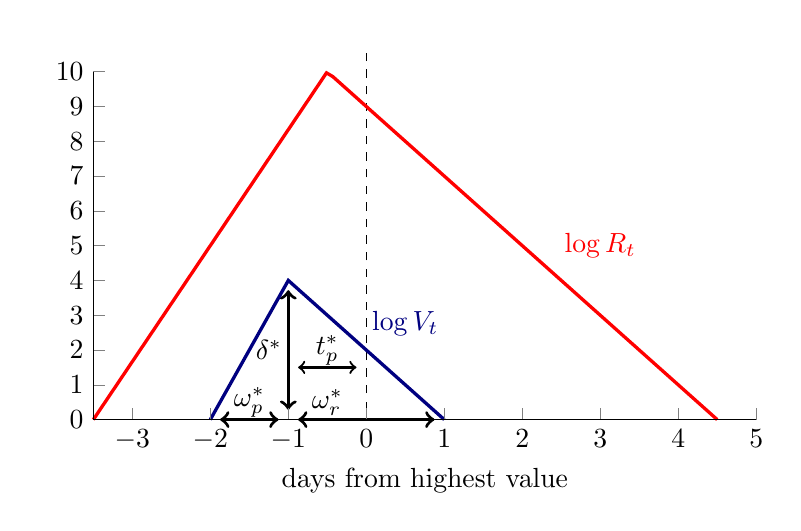
\begin{tikzpicture}
            \begin{axis}[
              no markers, domain=-3.5:4.5, samples=100,
              axis lines*=left, xlabel=days from highest value, ylabel=$ $,
              height=6cm, width=10cm,
              xtick={-5,-4,-3,-2,-1,0,1,2,3,4,5}, ytick={0,1,2,3,4,5,6,7,8,9,10},
              ymin = 0, ymax = 10, xmin =-3.5, xmax = 5,
              enlargelimits=false, clip=false, axis on top,
              grid = none, name=onset,
              declare function={
                pefunc(\x)=(\x <= -0.5) * (10 / 3 * (\x + 3.5))  +
                 (\x > -0.5) * (10 - 10 / 5 * (\x + 0.5));
                pefunc2(\x)=(\x <= -1) * (4 / 1 * (\x + 2))  +
                 (\x > -1) * (4 - 4 / 2 * (\x + 1));
              }
              ]
              % \addplot [draw=none, fill=blue!20] {lnormal(1.75,0.33)}\closedcycle;
              % \addplot [very thick, blue!50!black] {lnormal(1.75,0.33)};
            %   \addplot [draw=none, fill=orange!20] {gammapdf(4, 1)}\closedcycle;
            %   \addplot [very thick, orange!50!black] {gammapdf(4, 1)};
           
              \node (a) at (axis cs: -0.5,0) { };
              \node (a0) at (axis cs: -1,0) { };
              \node (b) at (axis cs: -1,4) { };
              \node (c) at (axis cs: -0.5,10) { };
              \node (d) at (axis cs: -2,0) { };
              \node (e) at (axis cs: 1,0) { };
              \node (f) at (axis cs: -3.5,0) { };
              \node (g) at (axis cs: 4.5,0) { };
              \node (h) at (axis cs: 0,0) { };
              \node (i) at (axis cs: 0,11) { };
              \node (j) at (axis cs: -1,1.5) { };
              \node (k) at (axis cs: 0,1.5) { };
              \draw[<->, very thick](a0)--(b);
              % \draw[<->, very thick](a)--(c);
              \draw[<->, very thick](a0)--(d);
              \draw[<->, very thick](a0)--(e);
              % \draw[<->, very thick](a)--(f);
              % \draw[<->, very thick](a)--(g);
               \draw[-, dashed](h)--(i);
              \draw[<->, thick](j)--(k);
              \node at (axis cs: -0.5,0.5) {$\omega^*_r$};
              % \node at (axis cs: 2,0.5) {$\omega_r$};
              \node at (axis cs: -1.5,0.5) {$\omega^*_p$};
              \node at (axis cs: -0.5,2) {$t^*_p$};
              % \node at (axis cs: -2.5,0.5) {$\omega_p$};
              \node at (axis cs: -1.25,2) {$\delta^*$};
              % \node at (axis cs: -0.75,6) {$\delta$};
              \addplot [very thick, red] {pefunc(x)};
              \addplot [very thick, blue!50!black, domain =-2:1] {pefunc2(x)};
              \node[red] at (axis cs: 3,5) {$\log R_t$};
              \node[blue!50!black] at (axis cs: 0.5,2.75) {$\log V_t$};
            \end{axis}
        \end{tikzpicture}
        \label{fig:illustration2}
    \end{figure}
    
\section{Computation}
All models are implemented in Stan and fit using the No-U-Turn Sampler (NUTS), a variant of Hamiltonian Monte Carlo, via the \texttt{cmdstanr} interface to CmdStan. We run 4 parallel chains, each with 1{,}000 warmup iterations and 2{,}000 sampling iterations, yielding 8{,}000 posterior draws in total. We set the target acceptance probability to $\delta_{\text{adapt}} = 0.95$ (the NUTS \texttt{adapt\_delta} parameter) to reduce the incidence of divergent transitions, which can signal numerical instability in regions of high curvature. The entire pipeline is orchestrated using the \texttt{targets} package for R, which manages dependency tracking, caching, and reproducibility.

Several computational strategies are employed to improve sampling efficiency. First, all individual-level random effects use a non-centered parameterization (NCP), in which standard normal auxiliary variables $\mathbf{z}_i$ are sampled and then scaled by the relevant standard deviations in the transformed parameters block. This eliminates the funnel geometries that arise from centered parameterizations of hierarchical models. For the correlated RNA random effects, the NCP is extended via the Cholesky factorization of the correlation matrix (Section 3.6), which parameterizes the correlation structure through its lower-triangular factor $\mathbf{L}$ and avoids direct sampling of the positive-definite matrix $\boldsymbol{\Omega}$. Second, the smooth trajectory function (Section 3.1) provides continuously differentiable log-densities, which are better suited to the leapfrog integrator used by HMC than the piecewise function with its non-differentiable kink at the peak. Third, population-level kinetic parameters (peak height, proliferation time, clearance time, flat-top duration) are parameterized on a non-centered log scale with prior mean and coefficient of variation supplied as data, which standardizes the posterior geometry and reduces sensitivity to the prior scale.

Convergence is assessed using the split-$\hat{R}$ statistic, with all parameters required to satisfy $\hat{R} < 1.01$, and effective sample sizes (both bulk and tail ESS). We additionally monitor the number of divergent transitions and inspect trace plots for key parameters. Model comparison is performed using Pareto-smoothed importance sampling leave-one-out cross-validation (PSIS-LOO) computed from the observation-level log-likelihoods stored in the \texttt{generated quantities} block, supplemented by the widely applicable information criterion (WAIC). Posterior predictive checks are conducted by drawing replicated datasets from the fitted model and comparing their summary statistics to the observed data.

\section{Model checking and inference}

\section{Results}

\subsection{Predicting individual trajectories}

\subsection{Determining optimal quarantine or isolation policies}

There are two key determinants of whether an isolation policy will be effective: 1) can infected individuals be identified early in the infectious phase and 2) once identified how long must they remain isolated. Both can be informed by a proper model. 

\begin{figure}[p]
    \centering
    
\includegraphics[width=\linewidth]{../3_figures/probability.png}
    \caption{}
\end{figure}

\begin{figure}[p]
    \centering
    
\includegraphics[width=\linewidth]{../3_figures/probability_by_rapid_result.png}
    \caption{}
\end{figure}

\subsection{Inferring population parameters}

\subsection{Parameterizing transmission models}



\section{Discussion}

% \printbibliography

\clearpage
% ============================================================================
% SUPPLEMENT CONFIGURATION
% ============================================================================
% Change the prefix to adapt to journal requirements:
%   "A" for Appendix (default), "S" for Supplement, "SI" for Supporting Info
\newcommand{\suppprefix}{S}
% Figure path: change to point to journal-specific directory when using
% save_journal_figure() output (e.g., "../../output/figures/pnas")
\newcommand{\suppfigpath}{../../output/figures/pnas}
% Page numbering: set to 0 to restart, or comment out to continue from main text
\setcounter{page}{0}

\begin{appendix}

    \renewcommand{\thefigure}{\suppprefix\arabic{figure}}
    \setcounter{figure}{0}

    \renewcommand{\thetable}{\suppprefix\arabic{table}}
    \setcounter{table}{0}

    \renewcommand{\theequation}{\suppprefix\arabic{equation}}
    \setcounter{equation}{0}

    \renewcommand{\thesection}{\suppprefix\arabic{section}}
    \setcounter{section}{0}

    % -------------------------------------------------------------------
    % Title page
    % -------------------------------------------------------------------
    \newpage
    \begin{center}
        {\Large \textbf{Supplementary Materials}} \\[0.5em]
        {\large Inferring infectiousness: a joint model of the within-host viral kinetics of SARS-CoV-2} \\[0.5em]
        %Christopher Boyer and Marc Lipsitch \\[1em]
        \today
    \end{center}
    \vspace{1em}

    \noindent This supplement contains prior predictive checks (Section~\ref{sec:supp_prior}), a comparison of the semi-mechanistic trajectory model to the target cell limited ODE (Section~\ref{sec:supp_tcl}), a description of the flat-top trajectory extension (Section~\ref{sec:supp_flattop}), convergence diagnostics (Section~\ref{sec:supp_convergence}), individual-level trajectory fits for each cohort (Section~\ref{sec:supp_fits}), posterior predictive checks (Section~\ref{sec:supp_ppc}), the parameter recovery simulation study (Section~\ref{sec:supp_recovery}), additional parameter estimates including covariate effects, the RNA-to-PFU transformation, and the individual random effect correlation structure (Section~\ref{sec:supp_params}), and covariate-stratified probability curves for testing and isolation policy (Section~\ref{sec:supp_strat}).

    % ===================================================================
    % SECTION 1: PRIOR PREDICTIVE CHECKS
    % ===================================================================
    \section{Prior predictive checks} \label{sec:supp_prior}

    Figures~\ref{fig:prior_pe}--\ref{fig:prior_sym} display draws from the joint prior distribution of model parameters before conditioning on data, illustrating the range of trajectories and derived quantities consistent with the prior specification described in Section~\ref{sec:priors} of the main text.

    \begin{figure}[p]
        \centering
        \includegraphics[width=\linewidth]{\suppfigpath/prior_pe.pdf}
        \caption[Prior predictive: RNA trajectory parameters]{Prior predictive check for the piecewise exponential trajectory parameters. Each panel shows 500 draws from the marginal prior distribution of a single kinetic parameter (peak height $\delta$, proliferation duration $\omega_p$, clearance duration $\omega_r$, peak timing $t_p$), illustrating the range of values admitted by the prior before observing data. Gray shading indicates the approximate range observed in the literature.}
        \label{fig:prior_pe}
    \end{figure}

    \begin{figure}[p]
        \centering
        \includegraphics[width=\linewidth]{\suppfigpath/prior_trans_pe.pdf}
        \caption[Prior predictive: RNA-to-PFU transformation]{Prior predictive check for the log-affine RNA-to-PFU transformation parameters. Each panel shows draws from the joint prior of the intercept ($a_0$) and elasticity ($a_1$) parameters linking infectious virus trajectory parameters to viral RNA trajectory parameters. The elasticity prior is centered at 1 (proportional scaling) with positivity enforced by truncation.}
        \label{fig:prior_trans}
    \end{figure}

    \begin{figure}[p]
        \centering
        \includegraphics[width=\linewidth]{\suppfigpath/prior_trajectories.pdf}
        \caption[Prior predictive: trajectory draws]{Prior predictive trajectories. Two-dimensional kernel density estimate of simulated viral trajectories drawn from the joint prior distribution of all kinetic parameters, including population-level parameters, individual random effects, and the log-affine RNA-to-PFU transformation. Left panel: viral RNA; right panel: infectious virus (PFU). The y-axis is constrained to 0--25 log copies/mL to match the observed data range. The density illustrates the range and concentration of kinetic profiles implied by the prior before conditioning on data.}
        \label{fig:prior_traj}
    \end{figure}

    \begin{figure}[p]
        \centering
        \includegraphics[width=\linewidth]{\suppfigpath/prior_sym.pdf}
        \caption[Prior predictive: symptom onset model]{Prior predictive check for the discrete-time cloglog symptom onset model. Prior draws of the daily hazard of symptom onset as a function of days since infection, illustrating the range of onset timing and cumulative incidence curves consistent with the prior specification. The prior intercept is centered at $\zeta_0 = -3$ (corresponding to a ${\sim}5\%$ baseline daily hazard), with positive viral load effects $\zeta_1, \zeta_2 \sim N^+(0, 0.5)$ and post-peak sigmoid coefficients $\zeta_3, \zeta_4 \sim N(0, 1)$.}
        \label{fig:prior_sym}
    \end{figure}

    % ===================================================================
    % SECTION 2: TARGET CELL LIMITED MODEL COMPARISON
    % ===================================================================
    \section{Comparison with target cell limited model} \label{sec:supp_tcl}

    The semi-mechanistic piecewise exponential trajectory model (Section~3 of the main text) is motivated by the phenomenological similarity between its trajectory shape and the numerical solution of the target cell limited (TCL) ODE. Figures~\ref{fig:tcl_1}--\ref{fig:tcl_2} illustrate this correspondence by overlaying a least-squares--fitted smooth piecewise exponential approximation (Equation~3 of the main text) on the ODE solution for two model configurations, demonstrating that the semi-mechanistic model captures the salient features---exponential growth, peak, and exponential decline---while directly parameterizing the quantities of clinical interest.

    \begin{figure}[p]
        \centering
        \includegraphics[width=\linewidth]{\suppfigpath/tcl_example_1.pdf}
        \caption[TCL comparison: standard model]{Comparison between the standard target cell limited ODE solution (solid blue line; $\beta = 2.4 \times 10^{-5}$, $\delta = 2.0$, $\pi = 1700$, $c = 10$, $T_0 = 4 \times 10^8$, $V_0 = 0.4$) and a smooth piecewise exponential approximation fitted by least squares (dashed red line). The piecewise model closely tracks the exponential proliferation and clearance phases; the main discrepancy is a slight geometric mismatch near the rounded ODE peak versus the smooth log-sum-exp cap of the piecewise model.}
        \label{fig:tcl_1}
    \end{figure}

    \begin{figure}[p]
        \centering
        \includegraphics[width=\linewidth]{\suppfigpath/tcl_example_2.pdf}
        \caption[TCL comparison: refractory compartment]{As Figure~\ref{fig:tcl_1}, but for an extended TCL model that includes a refractory cell compartment ($\phi = 1$, $\rho = 0.5$; all other parameters identical). The innate immune response modeled by the refractory state produces a blunted, asymmetric trajectory with a faster initial decline followed by a prolonged tail. The piecewise exponential approximation captures the dominant features of this more complex ODE solution, supporting its use as a tractable reduced-form model even when the underlying biology includes additional compartments.}
        \label{fig:tcl_2}
    \end{figure}

    % ===================================================================
    % SECTION 3: FLAT-TOP TRAJECTORY EXTENSION
    % ===================================================================
    \section{Flat-top trajectory extension} \label{sec:supp_flattop}

    The smooth trajectory function used in the main text (Section~3.1) assumes that the viral load profile transitions immediately from proliferation to clearance at the peak. In reality, some individuals may exhibit an approximate plateau near peak viral load, during which infectious virus production and immune-mediated clearance are roughly balanced. To accommodate this possibility, we consider a generalized smooth trajectory that introduces a \emph{flat-top duration} parameter $\omega_f \geq 0$:
    \begin{equation}
        g_s(t; \theta) = \delta + \log \frac{a + b}{b \exp(-a(t - t_p)) + a \exp(b(t - (t_p + \omega_f)))} \label{eq:flattop}
    \end{equation}
    where $a = \delta / \omega_p$ and $b = \delta / \omega_r$ are the proliferation and clearance rates, as in the main text. When $\omega_f = 0$, this reduces to the standard smooth two-arm envelope used in our primary analysis. For $\omega_f > 0$, the rising and falling exponential arms are separated by $\omega_f$ days, producing an approximate plateau of width $\omega_f$ around the peak.

    However, when $\omega_f > 0$, the log-sum-exp envelope can overshoot the peak value $\delta$---an inherent artifact of merging two separated exponential arms. To prevent this, we apply a soft cap:
    \begin{equation}
        \tilde{g}_s(t; \theta) = g_s(t; \theta) - \frac{1}{\kappa}\log\!\left(1 + \exp\!\left(\kappa \left(g_s(t; \theta) - \delta\right)\right)\right) \label{eq:softcap}
    \end{equation}
    where $\kappa = 10$ controls the sharpness of the cap. This ensures $\tilde{g}_s \leq \delta$ everywhere while maintaining smooth gradients.

    When the flat-top extension is used, $\omega_f$ is shared between the RNA and PFU trajectories, and the parameter vector becomes $\theta = (\delta, \omega_p, \omega_r, t_p, \omega_f)$ for RNA and $\theta' = (\delta', \omega'_p, \omega'_r, t'_p, \omega_f)$ for PFU. Individual and source-level effects on $\omega_f$ are modeled independently (not included in the correlated random effect block) to keep the dimensionality of the Cholesky factor manageable.

    \paragraph{Model comparison.} Our implementation includes a compile-time toggle (\texttt{use\_wf}) that enables or disables the flat-top extension. In preliminary fits with $\omega_f$ enabled, the posterior for $\omega_f$ concentrated near zero, indicating that the data do not support a plateau phase beyond what is already captured by the smooth peak geometry. Formally, the model with $\omega_f = 0$ (the specification used in the main text) was preferred on the basis of WAIC, and the remaining parameter estimates were substantively unchanged. We therefore use the simpler specification without the flat-top parameter throughout the main analysis.

    % ===================================================================
    % SECTION 4: CONVERGENCE DIAGNOSTICS
    % ===================================================================
    \section{Convergence diagnostics} \label{sec:supp_convergence}

    \begin{figure}[p]
        \centering
        \includegraphics[width=\linewidth]{\suppfigpath/trace_plots.pdf}
        \caption[MCMC trace plots]{MCMC trace plots for key population-level parameters across all four chains. Each panel shows the sampled values for one parameter as a function of iteration number, with chains distinguished by color. All parameters show good mixing with no visible trends, multimodality, or stuck chains, consistent with the split-$\hat{R}$ values reported in Section~\ref{sec:model_checking} of the main text.}
        \label{fig:trace}
    \end{figure}

    % ===================================================================
    % SECTION 5: INDIVIDUAL TRAJECTORY FITS
    % ===================================================================
    \section{Individual trajectory fits} \label{sec:supp_fits}

    Figures~\ref{fig:fit_ataccc}--\ref{fig:fit_legacy} show individual-level trajectory fits for all participants in each of the five cohorts. For each individual, the posterior median viral RNA trajectory (blue line) with 95\% credible interval (blue ribbon) is overlaid on observed qPCR-derived log RNA concentrations (blue points). Where available, the posterior median infectious virus (PFU) trajectory (red line) with 95\% credible interval (red ribbon) is shown with observed culture-based measurements (red points). Predicted lateral flow device (LFD) positivity probabilities are displayed as shaded tiles (green = positive, gray = negative), and observed symptom onset is indicated by markers. The limit of detection for each assay is shown as a horizontal dashed line.

    \begin{landscape}
        \begin{figure}[p]
            \centering
            \includegraphics[width=\linewidth]{\suppfigpath/ataccc_fit.pdf}
            \caption[ATACCC individual fits]{Individual trajectory fits for all 57 ATACCC participants. This cohort provides the most complete multi-modal data, with paired qPCR, viral culture, LFD, and symptom diary observations at each time point, enabling direct comparison of all four observation models within each individual.}
            \label{fig:fit_ataccc}
        \end{figure}

        \begin{figure}[p]
            \centering
            \includegraphics[width=\linewidth]{\suppfigpath/nba_fit.pdf}
            \caption[NBA individual fits]{Individual trajectory fits for selected NBA participants. This cohort contributes only qPCR data; the infectious virus trajectory (red) is inferred entirely through the hierarchical RNA-to-PFU transformation and the population prior on PFU kinetics, illustrating the model's ability to impute unobserved infectious virus dynamics from RNA data alone.}
            \label{fig:fit_nba}
        \end{figure}

        \begin{figure}[p]
            \centering
            \includegraphics[width=\linewidth]{\suppfigpath/uiuc_fit.pdf}
            \caption[UIUC individual fits]{Individual trajectory fits for all 60 UIUC participants. Like ATACCC, this cohort has multi-modal data (qPCR, TCID$_{50}$ culture, LFD, symptoms), with the TCID$_{50}$ culture results modeled via the mechanistic interval-censored normal observation model described in Section~3.4 of the main text.}
            \label{fig:fit_uiuc}
        \end{figure}

        \begin{figure}[p]
            \centering
            \includegraphics[width=\linewidth]{\suppfigpath/hct_fit.pdf}
            \caption[HCT individual fits]{Individual trajectory fits for all 18 Human Challenge Trial participants. The known inoculation time ($t=0$) provides a fixed reference point absent in observational cohorts, enabling precise estimation of the proliferation phase duration and timing. PFU and FFA culture measurements are available for all time points.}
            \label{fig:fit_hct}
        \end{figure}

        \begin{figure}[p]
            \centering
            \includegraphics[width=\linewidth]{\suppfigpath/legacy_fit.pdf}
            \caption[Legacy individual fits]{Individual trajectory fits for all 157 Crick Legacy participants. This cohort contributes qPCR and symptom onset data but no viral culture or LFD results. The model uses the joint structure and hierarchical prior to impute the infectious virus trajectory from RNA data and the estimated population-level RNA-to-PFU transformation. All participants are vaccinated (2 or 3 doses), and infections span the Delta and Omicron waves.}
            \label{fig:fit_legacy}
        \end{figure}
    \end{landscape}

    % ===================================================================
    % SECTION 6: POSTERIOR PREDICTIVE CHECKS
    % ===================================================================
    \section{Posterior predictive checks} \label{sec:supp_ppc}

    Figures~\ref{fig:ppc_rna}--\ref{fig:ppc_sym} display posterior predictive checks comparing simulated replicated data from the fitted model to the observed data across all four assay types, both in aggregate and stratified by cohort. Replicated datasets are generated by drawing from the posterior predictive distribution at each observed time point for each individual.

    \begin{figure}[p]
        \centering
        \includegraphics[width=\linewidth]{\suppfigpath/ppc_rna.pdf}
        \caption[PPC: viral RNA]{Posterior predictive check for viral RNA (qPCR) observations. The distribution of observed log RNA concentrations (black density curve) is compared to 100 replicated datasets drawn from the posterior predictive distribution (coloured density curves). Agreement between observed and replicated distributions indicates adequate model fit for the RNA observation model.}
        \label{fig:ppc_rna}
    \end{figure}

    \begin{figure}[p]
        \centering
        \includegraphics[width=\linewidth]{\suppfigpath/ppc_rna_cohort.pdf}
        \caption[PPC: viral RNA by cohort]{Posterior predictive check for viral RNA, stratified by cohort. Each panel shows the observed versus replicated RNA distribution for a single cohort. The model captures differences in the marginal RNA distributions across cohorts, including the broader distribution in the NBA cohort (which has the most individuals) and the more concentrated distributions in the smaller cohorts.}
        \label{fig:ppc_rna_cohort}
    \end{figure}

    \begin{figure}[p]
        \centering
        \includegraphics[width=\linewidth]{\suppfigpath/ppc_pfu.pdf}
        \caption[PPC: infectious virus]{Posterior predictive check for infectious virus (PFU/TCID$_{50}$/FFA) observations. The observed distribution of log$_{10}$ PFU/mL values is shown as a black density curve, overlaid with density curves from 100 replicated datasets drawn from the posterior predictive distribution. Close overlap between the observed and replicated densities indicates that the PFU observation model adequately captures the location, spread, and shape of the culture-based measurements.}
        \label{fig:ppc_pfu}
    \end{figure}

    \begin{figure}[p]
        \centering
        \includegraphics[width=\linewidth]{\suppfigpath/ppc_pfu_cohort.pdf}
        \caption[PPC: infectious virus by cohort]{Posterior predictive check for infectious virus, stratified by cohort. Panels show results for the three cohorts with culture data (ATACCC, UIUC, HCT). The model accommodates differences in PFU distributions across cohorts arising from different culture assay types (viral culture, TCID$_{50}$, PFU/FFA).}
        \label{fig:ppc_pfu_cohort}
    \end{figure}

    \begin{figure}[p]
        \centering
        \includegraphics[width=\linewidth]{\suppfigpath/ppc_lfd_calibration.pdf}
        \caption[PPC: LFD calibration]{Calibration plot for the lateral flow device (LFD) observation model. Predicted LFD positivity probabilities are binned into deciles; within each bin, the observed LFD-positive frequency ($y$-axis) is plotted against the mean predicted probability ($x$-axis), with 95\% binomial confidence intervals (vertical bars) and the number of observations per bin labeled above each point. The dashed diagonal line represents perfect calibration. Points falling near the diagonal indicate that the logistic LFD model is well calibrated across the full range of predicted positivity.}
        \label{fig:ppc_lfd}
    \end{figure}

    \begin{figure}[p]
        \centering
        \includegraphics[width=\linewidth]{\suppfigpath/ppc_lfd_calibration_cohort.pdf}
        \caption[PPC: LFD calibration by cohort]{Calibration plot for the LFD observation model, stratified by cohort. Panels show results for the three cohorts with LFD data (ATACCC, UIUC, HCT). Calibration is maintained across cohorts despite differences in sampling frequency and LFD assay conditions.}
        \label{fig:ppc_lfd_cohort}
    \end{figure}

    \begin{figure}[p]
        \centering
        \includegraphics[width=\linewidth]{\suppfigpath/ppc_lfd_calibration_phase.pdf}
        \caption[PPC: LFD calibration by infection phase]{Calibration plot for the LFD observation model, stratified by infection phase (pre-peak versus post-peak viral RNA). Pre-peak observations (time $\leq 0$ relative to observed RNA peak) show lower observed LFD positivity than predicted at comparable predicted probability levels, consistent with the lag between viral replication and antigen accumulation to the LFD detection threshold reported by~\cite{hakki2022onset}. Post-peak observations are well calibrated along the diagonal. This asymmetry reflects a biologically expected feature: during viral proliferation, RNA levels rise faster than antigen protein concentrations, leading to lower LFD sensitivity for a given predicted positivity level than during the clearance phase.}
        \label{fig:ppc_lfd_phase}
    \end{figure}

    \begin{figure}[p]
        \centering
        \includegraphics[width=\linewidth]{\suppfigpath/ppc_sym.pdf}
        \caption[PPC: symptom onset]{Posterior predictive check for symptom onset. The observed Kaplan--Meier cumulative incidence curve of symptom onset (black step function) is compared to cumulative incidence curves from 200 replicated datasets drawn from the posterior predictive distribution of the discrete-time complementary log-log hazard model (coloured lines, with 95\% pointwise credible band shaded). For each replicated dataset, symptom onset is simulated by drawing Bernoulli outcomes at each at-risk day using the posterior predictive hazard probability. Agreement between the observed and replicated cumulative incidence indicates that the symptom onset model adequately captures the timing and proportion of symptomatic infections.}
        \label{fig:ppc_sym}
    \end{figure}

    \begin{figure}[p]
        \centering
        \includegraphics[width=\linewidth]{\suppfigpath/ppc_sym_cohort.pdf}
        \caption[PPC: symptom onset by cohort]{Posterior predictive check for symptom onset, stratified by cohort. Panels show cumulative incidence of symptom onset for the four cohorts with symptom data (ATACCC, UIUC, HCT, Legacy). Per-cohort agreement between observed and replicated cumulative incidence curves indicates that the symptom model captures cohort-level differences in symptom onset timing and overall symptomatic fraction.}
        \label{fig:ppc_sym_cohort}
    \end{figure}

    % ===================================================================
    % SECTION 7: PARAMETER RECOVERY
    % ===================================================================
    \section{Parameter recovery} \label{sec:supp_recovery}

    \begin{figure}[p]
        \centering
        \includegraphics[width=\linewidth]{\suppfigpath/param_recovery.pdf}
        \caption[Parameter recovery]{Parameter recovery from simulated data. A synthetic dataset was generated from the model's prior predictive distribution using a 50\% random subsample of the observed covariate and missingness structure, and the model was refit to the simulated data. For each of 34 assessed parameters, the true generating value (horizontal line) is compared to the posterior 95\% credible interval from the recovery fit (vertical bar with point at the median). Covered parameters (true value within the 95\% CrI) are shown in blue; non-covered parameters are shown in red. Overall coverage is 76.5\% (26/34). Non-covered parameters ($\sigma_{\text{pfu}}$, $\hat\lambda_{\text{fp}}$, $\hat\lambda_{\text{fn}}$, $\alpha_{\text{cult},1}$, and three others) are discussed in Section~\ref{sec:model_checking} of the main text.}
        \label{fig:recovery}
    \end{figure}

    % ===================================================================
    % SECTION 8: ADDITIONAL PARAMETER ESTIMATES
    % ===================================================================
    \section{Additional parameter estimates} \label{sec:supp_params}

    \subsection{Covariate effects on RNA kinetics}

    Tables~\ref{tab:cov_peak}--\ref{tab:cov_clearance} report the full posterior estimates of covariate effects on each RNA kinetic parameter. Effects are expressed as $\exp(\beta)$, representing the multiplicative fold change in the kinetic parameter relative to the reference category (unvaccinated, immunologically na\"ive, 0--30 year old with pre-Alpha variant). Values greater than 1 indicate an increase relative to the reference; values less than 1 indicate a decrease. These results are summarized visually in Figure~\ref{fig:covariates} of the main text.

    \input{../../output/tables/supp_cov_peak.tex}
    \input{../../output/tables/supp_cov_prolif.tex}
    \input{../../output/tables/supp_cov_clearance.tex}

    \subsection{RNA-to-PFU transformation and correlation structure}

    Figure~\ref{fig:corr_densities} shows the marginal posterior densities for each element of the RNA individual random effect correlation matrix, and Figure~\ref{fig:corr_matrix} displays the full posterior median correlation matrix with uncertainty. These supplement the summary in Section~8.5 and Figure~\ref{fig:correlations} of the main text.

    \begin{figure}[p]
        \centering
        \includegraphics[width=\linewidth]{\suppfigpath/corr_densities.pdf}
        \caption[RNA RE correlation densities]{Marginal posterior densities for each pairwise correlation among the four RNA individual random effects (peak timing $t_p$, peak height $\delta$, proliferation duration $\omega_p$, clearance duration $\omega_r$). Each panel shows the posterior density (filled curve) with the prior density (dashed line) overlaid for comparison. The shift between prior and posterior indicates the direction and degree of data learning for each correlation.}
        \label{fig:corr_densities}
    \end{figure}

    \begin{figure}[p]
        \centering
        \includegraphics[width=\linewidth]{\suppfigpath/corr_matrix.pdf}
        \caption[RNA RE correlation matrix]{Posterior median correlation matrix of the RNA individual random effects, displayed as a heatmap. Colors indicate the sign and magnitude of each pairwise correlation: blue tones represent negative correlations and red tones represent positive correlations. Numeric values show the posterior median; 95\% credible intervals are reported in Section~8.5 of the main text.}
        \label{fig:corr_matrix}
    \end{figure}

    \input{../../output/tables/supp_transformation.tex}

    \subsection{Individual random effect standard deviations}

    Table~\ref{tab:re_sd} reports the posterior estimates of individual-level random effect standard deviations for both the RNA and PFU trajectories. Larger values indicate greater between-individual variability in that kinetic parameter.

    \input{../../output/tables/supp_re_sd.tex}

    \subsection{Observation model parameters}

    Tables~\ref{tab:lfd} and~\ref{tab:symptom} report the posterior estimates of the LFD and symptom onset observation model parameters, respectively. Both models include smooth post-peak sigmoid interaction terms that allow the relationship between viral load and the outcome to differ between the proliferation and clearance phases: the LFD model uses a logistic link (Section~3.3 of the main text) and the symptom model uses a discrete-time complementary log-log hazard (Section~3.5).

    \input{../../output/tables/supp_lfd.tex}
    \input{../../output/tables/supp_symptom.tex}

    \subsection{Stratified probability curves by covariate profile}
    \label{sec:supp_strat}

    Figure~\ref{fig:strat_curves} shows the probability of remaining culture-positive and LFD-positive as a function of days since first positive PCR, stratified by covariate profile. These curves supplement the marginal (population-averaged) probability curves presented in Figure~\ref{fig:probability_curves} of the main text by illustrating how variant, vaccination status, and infection history modulate the duration of infectiousness. Profiles are selected to maximise visual contrast and include the Reference (unvaccinated, pre-Alpha, first infection, age $<$30), single-factor profiles (Boosted, Reinfection, Delta, Omicron, Age 50+), and composite profiles (Boosted + Omicron 2022, Unboosted + Delta 2021).

    \begin{landscape}
    \begin{figure}[p]
        \centering
        \includegraphics[width=\linewidth]{\suppfigpath/figS_stratified_curves.pdf}
        \caption[Stratified probability curves]{Probability of remaining culture-positive \textbf{(A)} and LFD-positive \textbf{(B)} as a function of days since first positive PCR test, stratified by covariate profile. Points show posterior median probabilities at each integer day; vertical bars show 95\% credible intervals. Profiles are horizontally dodged for readability. The Reinfection profile clears fastest, consistent with anamnestic immunity accelerating viral clearance. The Boosted + Omicron (2022) profile shows the most prolonged culture positivity, reflecting the longer proliferation phase associated with both vaccination and Omicron. Culture and LFD positivity curves track each other closely across profiles, supporting the use of LFD as a proxy for infectious status regardless of covariate profile.}
        \label{fig:strat_curves}
    \end{figure}
    \end{landscape}

    \subsection{Serial rapid testing conditional on symptom onset}
    \label{sec:supp_serial_lfd}

    Figure~\ref{fig:conditional_symptom} shows the probability of remaining culture-positive conditional on lateral flow device (LFD) test outcomes, aligned to the day of symptom onset, for three representative covariate profiles (Reinfection, Reference, Boosted + Omicron 2022). In addition to conditioning on a single positive or negative LFD result, the figure includes a series conditioning on two consecutive negative LFD results (current day plus preceding day), quantifying the incremental reassurance provided by serial testing.

    \begin{landscape}
    \begin{figure}[p]
        \centering
        \includegraphics[width=\linewidth]{\suppfigpath/fig8_conditional_symptom.pdf}
        \caption[Conditional culture positivity by LFD outcome and symptom onset]{Probability of remaining culture-positive conditional on lateral flow device (LFD) test outcomes, as a function of days since symptom onset, for three representative covariate profiles. Points show posterior medians; vertical bars show 95\% credible intervals. Three conditions are compared: LFD positive (red), single LFD negative (blue), and two consecutive LFD negatives --- current day plus preceding day (green). Two consecutive negative results provide substantially greater reassurance than a single negative, particularly in the day 5--10 window where the single-negative false reassurance rate remains appreciable. Dashed vertical lines indicate days 5 and 10.}
        \label{fig:conditional_symptom}
    \end{figure}
    \end{landscape}

    \section{Anatomical site-specific sampling and pooling model}
    \label{sec:supp_site}

    \subsection{Motivation}

    The five cohorts in this study differ in their upper respiratory tract sampling protocols. Three cohorts (ATACCC, NBA, Legacy) combine nasal and oropharyngeal swabs into a single collection tube prior to PCR, yielding one RNA concentration measurement per time point that reflects a \emph{pooled} sample from both anatomical sites. Two cohorts (HCT, UIUC) collect site-specific specimens --- nasal and throat swabs (HCT) or nasal and saliva samples (UIUC) --- that are processed separately, providing distinct RNA concentration measurements from each site.

    In the current model, site-specific measurements from HCT and UIUC are combined prior to model fitting by taking the arithmetic mean on the linear scale: $R_{\text{obs}} = \log\bigl(\tfrac{1}{2}e^{R_n} + \tfrac{1}{2}e^{R_t}\bigr)$, where $R_n$ and $R_t$ denote the log RNA concentrations from the nasal and throat sites, respectively. While this produces a single summary value per time point, the averaging has two drawbacks. First, it discards information about site-specific kinetic differences --- for example, whether the nose or throat leads in proliferation or clears virus faster. Second, it introduces a subtle inconsistency with the PFU likelihood, which uses \emph{throat-only} culture data (the only site from which viable virus was assayed in HCT).

    Figure~\ref{fig:site_comparison}A illustrates this issue using data from three representative HCT participants. The nasal and throat RNA trajectories can differ substantially in timing and magnitude, yet the current model receives only their average. The throat-only PFU measurements (orange triangles) align with the throat trajectory but may diverge from the nose trajectory, particularly during the early proliferation phase when viral replication in the nose may precede the throat.

    \subsection{Chemistry of swab pooling}

    When two swabs at concentrations $C_n$ and $C_t$ (copies/mL) are pooled into a single tube, the resulting measured concentration is a weighted sum:
    \begin{equation}
        C_{\text{pool}} = w_n C_n + w_t C_t, \quad w_n + w_t = 1,
        \label{eq:pool_linear}
    \end{equation}
    where $w_n$ and $w_t$ reflect the relative collection efficiencies (encompassing swab absorption capacity, elution volume, and extraction efficiency at each anatomical site). On the natural-log scale, this becomes:
    \begin{equation}
        R_{\text{pool}} = \operatorname{log\_sum\_exp}\!\bigl(R_n + \alpha_n,\; R_t + \alpha_t\bigr),
        \label{eq:pool_log}
    \end{equation}
    where $\alpha_s = \log w_s$ for $s \in \{n, t\}$ are log-scale collection-efficiency weights. This is numerically stable and can be computed directly in Stan using the built-in \texttt{log\_sum\_exp} function.

    The current averaging procedure implicitly assumes equal weights ($w_n = w_t = 0.5$, i.e.\ $\alpha_n = \alpha_t = \log 0.5$). A site-specific extension would estimate $\alpha_n$ and $\alpha_t$ from data, allowing the model to learn whether one site dominates the pooled signal.

    \subsection{Site-specific trajectory model}

    A natural extension is to model each anatomical site $s \in \{n, t\}$ as having its own latent RNA trajectory, derived from the individual's shared infection process but offset by site-specific parameters:
    \begin{align}
        \tau_{p,s} &= \tau_p + \delta_\tau^{(s)}, &
        d_{p,s} &= d_p + \delta_d^{(s)}, \nonumber \\
        \omega_{p,s} &= \omega_p + \delta_{\omega_p}^{(s)}, &
        \omega_{r,s} &= \omega_r + \delta_{\omega_r}^{(s)},
        \label{eq:site_offsets}
    \end{align}
    where $\delta_\cdot^{(s)}$ are population-level site offset parameters (with throat as the reference site, so $\delta_\cdot^{(t)} = 0$). The site-specific trajectory $R_s(t)$ is then computed using the same piecewise exponential function as the main model but evaluated at the site-shifted parameters.

    Figure~\ref{fig:site_comparison}B provides empirical support for this structure. The median log-difference between nasal and throat RNA ($R_n - R_t$) varies systematically over the course of infection, suggesting that the two sites do not simply differ by a constant offset but exhibit distinct kinetic profiles.

    \subsection{Likelihood structure}

    Under the site-specific extension, the RNA likelihood would depend on the cohort's sampling protocol:
    \begin{itemize}
        \item \textbf{Site-specific cohorts} (HCT, UIUC): Each site contributes an independent observation:
        \begin{equation}
            R_{s,\text{obs}} \sim \operatorname{Normal}\!\bigl(R_s(t),\; \sigma_{\text{rna}}\bigr), \quad s \in \{n, t\}.
        \end{equation}
        This doubles the number of RNA likelihood terms for these cohorts, providing substantially more information per time point.
        \item \textbf{Pooled cohorts} (ATACCC, NBA, Legacy): The observed pooled measurement follows from Equation~\eqref{eq:pool_log}:
        \begin{equation}
            R_{\text{obs}} \sim \operatorname{Normal}\!\bigl(R_{\text{pool}}(t),\; \sigma_{\text{rna}}\bigr),
        \end{equation}
        where $R_{\text{pool}}(t)$ is computed from the two site-specific trajectories and the estimated pooling weights.
    \end{itemize}
    The PFU likelihood would use the throat-specific trajectory $R_t(t)$ directly, eliminating the current inconsistency between averaged RNA and throat-only PFU data.

    \subsection{Implementation notes}

    This extension is fully compatible with the existing model architecture and could be controlled by a \texttt{use\_site\_model} flag (analogous to the existing \texttt{use\_smooth} and \texttt{use\_wf} flags). When disabled ($= 0$), the site offsets collapse to zero and the pooling weights to $w_n = w_t = 0.5$, recovering the current model exactly. When enabled ($= 1$), the model would estimate up to four site offset parameters ($\delta_\tau, \delta_d, \delta_{\omega_p}, \delta_{\omega_r}$) plus one free pooling weight parameter (since $\alpha_n + \alpha_t$ is determined by the softmax constraint). These are population-level parameters identifiable from the $\sim$18 HCT and $\sim$60 UIUC individuals with site-specific data.

    The data pipeline would expand site-specific observations into separate rows (one per site per time point) and add a site index to the Stan data. Site-specific limits of detection would also be required, since the LOD may differ between anatomical sites due to differences in swab type, collection technique, or assay calibration.

    \begin{figure}[p]
        \centering
        \includegraphics[width=\linewidth]{\suppfigpath/figS_site_comparison.pdf}
        \caption[Site-specific RNA trajectories in the HCT cohort]{\textbf{(A)} Nasal (blue) and throat (red) RNA concentration data (points) for three representative participants in the SARS-CoV-2 Human Challenge Study, with the arithmetic mean used in the current model shown as crosses. Smooth curves show smoothed piecewise exponential fits to each series independently: solid blue (nose), solid red (throat), dashed grey (average), and solid orange (PFU). Orange triangles show PFU measurements from throat-only viral culture. The two anatomical sites exhibit distinct kinetic profiles, with the nasal site often reaching higher peak concentrations and the PFU trajectory aligning more closely with the throat RNA than with the averaged signal. The current model's averaging obscures these site-specific differences. \textbf{(B)} Population-level median (shaded IQR) difference $\log(\text{RNA}_{\text{nose}}) - \log(\text{RNA}_{\text{throat}})$ across all HCT participants as a function of days since first positive test. The difference is not constant over time, supporting a model with site-specific kinetic offsets rather than a simple multiplicative correction. Bins with fewer than three observations are excluded.}
        \label{fig:site_comparison}
    \end{figure}

\section{Relationship between log-affine transformation and convolution}
\label{sec:supp_logaffine}

The log-affine transformation that maps RNA kinetic parameters to PFU kinetic parameters (Section~3.2 of the main text) can be motivated from the underlying biology. In the target cell limited model, viral RNA accumulates according to $dR/dt = qV_t - eR_t$, where $q$ is the RNA production rate per infectious virion and $e$ is the RNA degradation rate. The solution is the convolution
\begin{equation*}
    R_t = q \int_0^t e^{-e(t-s)} V_s\,ds.
\end{equation*}
For a piecewise exponential infectious virus trajectory $\log V_t = g(t; \theta)$ with proliferation rate $a = \delta/\omega_p$ and clearance rate $b = \delta/\omega_r$, the convolution can be evaluated in closed form on each arm.

\paragraph{Pre-peak ($t \leq t_p$).} On the rising arm, $V_t = V_0\,e^{at}$ and the convolution yields
\begin{equation*}
    R_t = \frac{q}{e + a}\,V_t
\end{equation*}
which is a pure scaling of the virus trajectory. Taking logarithms, $\log R_t = \log(q/(e+a)) + \log V_t$, which has the same functional form as the rising arm of a piecewise exponential with a log-additive offset to the peak height. The log-affine transformation captures this relationship exactly.

\paragraph{Post-peak ($t > t_p$).} On the falling arm, $V_t = V_p\,e^{-b(t-t_p)}$, and the convolution gives
\begin{equation*}
    R_t = \frac{q}{e - b}\,V_t + \frac{q(a + b)}{(e + a)(e - b)}\,V_p\,e^{-e(t-t_p)}
\end{equation*}
(assuming $e \neq b$). The first term tracks the virus with a scaling factor; the second is a ``memory'' term that decays at the RNA clearance rate $e$ rather than the viral clearance rate $b$. When $e > b$ (RNA clears faster than virus declines), the memory term decays rapidly and the log-affine transformation is an excellent approximation. When $e < b$ (RNA persists longer than virus, the typical biological scenario), the memory term dominates at late times, producing the characteristic delayed and broadened RNA clearance observed empirically.

\paragraph{Smooth trajectory.} For the smooth log-sum-exp trajectory $g_s(t)$, the convolution integral does not admit an elementary closed form---it reduces to a hypergeometric-type integral because the virus trajectory is a nonlinear function of two competing exponentials. However, the closed-form expressions for the piecewise trajectory are asymptotically correct far from the peak (where one exponential arm dominates), and the discrepancy is localized to a narrow region around the peak where both the virus and RNA concentrations are at their maximum and diagnostically least ambiguous. The log-affine transformation therefore provides a computationally tractable approximation that captures the dominant kinetic features---delayed peak and prolonged clearance of RNA relative to infectious virus---without requiring numerical quadrature or ODE integration inside the MCMC sampler (see Figure~\ref{fig:antigen_schematic}c--d).

\section{LFD observation model: indicator interaction and alternative approaches}
\label{sec:supp_lfd_deriv}

\subsection{Antigen dynamics and the proliferation--clearance asymmetry}

Lateral flow devices detect viral nucleocapsid protein (antigen), whose concentration $A_t$ follows the same production--clearance ODE as viral RNA (Section~\ref{sec:supp_logaffine}), but with virus rather than infected cells as the source:
\begin{equation*}
    \frac{dA}{dt} = \alpha_1 V_t - \alpha_2 A_t.
\end{equation*}
The ratio $A_t / V_t$ is not constant over the infection. On the rising arm, $A_t / V_t \approx \alpha_1 / (\alpha_2 + a)$; on the falling arm, $A_t / V_t \approx \alpha_1 / (\alpha_2 - b) + \text{memory term}$. Since $\alpha_2 + a > \alpha_2 - b$ (assuming $a, b > 0$ and $\alpha_2 > b$), the antigen-to-virus ratio is lower during proliferation than during clearance. This means that at a given viral load, antigen concentration is lower pre-peak than post-peak---the proliferation--clearance asymmetry that motivates the model extension.

\subsection{Adopted approach: smooth post-peak sigmoid interaction}

The LFD observation model uses a smooth sigmoid interaction to allow the relationship between viral load and LFD sensitivity to differ between the rising and falling phases of infection:
\begin{equation*}
    \text{logit}\,P(L_t^* = 1) = \gamma_0 + \gamma_1 \log R_t + \gamma_2 \log V_t + \gamma_3 \,\sigma_\kappa(t - t_p) + \gamma_4 \,\sigma_\kappa(t - t_p) \log R_t
\end{equation*}
where $t_p$ is the individual's estimated RNA peak time and $\sigma_\kappa(x) = \text{logit}^{-1}(\kappa x)$ is a smooth sigmoid with steepness $\kappa$ (fixed at 5, giving a transition width of approximately one day). The effective model for LFD sensitivity is approximately:
\begin{equation*}
    \text{logit}\,P(L_t^* = 1) \approx \begin{cases}
        \gamma_0 + \gamma_1 \log R_t + \gamma_2 \log V_t & \text{pre-peak} \\
        (\gamma_0 + \gamma_3) + (\gamma_1 + \gamma_4) \log R_t + \gamma_2 \log V_t & \text{post-peak}
    \end{cases}
\end{equation*}
This is a natural extension of the regression framework already used throughout the model. It requires no additional functions or numerical computation: the peak time $t_p$ is already estimated for each individual as part of the RNA trajectory. Because $t_p$ is a latent parameter estimated jointly with all other model parameters via Hamiltonian Monte Carlo, the smooth sigmoid is preferred over a hard indicator $\mathbbm{1}(t \geq t_p)$: the latter creates a discontinuity that zeroes out the gradient with respect to $t_p$, impeding the leapfrog integrator. With $\kappa = 5$, the sigmoid transitions from 0.01 to 0.99 over approximately one day, which is both biologically reasonable (the switch from proliferation to clearance is not instantaneous) and numerically well-behaved. Near the peak, LFD sensitivity is close to its maximum, so the precise transition shape is inconsequential for the binary LFD outcome.

\subsection{Alternative approaches considered}

We considered several alternative approaches to capturing the asymmetry (summarized in Table~\ref{tab:lfd_approaches} and Figure~\ref{fig:antigen_schematic}d):

\begin{table}[h]
\centering
\caption{Comparison of approaches for modeling phase-asymmetric LFD sensitivity.}
\label{tab:lfd_approaches}
\begin{tabular}{lcccc}
\toprule
 & Convolution & Log-affine & Indicator & Derivative \\
\midrule
Additional parameters & 2 ($\alpha_1, \alpha_2$) & 8 (log-affine) & 2 ($\gamma_3, \gamma_4$) & 1 ($\gamma_3$) \\
Closed form & No & Approximate & Yes & Yes \\
Compatible with \texttt{reduce\_sum} & No\textsuperscript{a} & Yes & Yes & Yes \\
Identifiable from binary data & Partially & Poorly & Yes & Yes \\
Discontinuity at peak & No & No & Yes\textsuperscript{b} & No \\
\bottomrule
\multicolumn{5}{l}{\textsuperscript{a}Requires quadrature or discrete recursion at each observation.} \\
\multicolumn{5}{l}{\textsuperscript{b}Negligible: binary data makes this practically undetectable.}
\end{tabular}
\end{table}

\paragraph{Full convolution.} The most principled approach would model $A_t$ explicitly via the convolution $A_t = \alpha_1 \int_0^t e^{-\alpha_2(t-s)} V_s\,ds$. For the piecewise trajectory, this has a closed form (Section~\ref{sec:supp_logaffine}). For the smooth trajectory used in practice, no elementary closed form exists; the integral would require numerical quadrature at each observation within each MCMC iteration, which is incompatible with Stan's \texttt{reduce\_sum} parallelism.

\paragraph{Log-affine antigen layer.} One could add a second log-affine transformation mapping PFU parameters to antigen parameters, producing a piecewise exponential antigen trajectory with 8 additional parameters. This approximates the convolution well in the tails but misses the post-peak shoulder. More importantly, with only binary LFD outcomes (no quantitative antigen measurements), the 8 additional parameters would be poorly identified.

\paragraph{Derivative-based approach.} An alternative to the sigmoid interaction is to replace $\gamma_3 \,\sigma_\kappa(t - t_p) + \gamma_4 \,\sigma_\kappa(t - t_p) \log R_t$ with a single term $\gamma_3 \dot{g}_s(t)$, where $\dot{g}_s(t)$ is the time derivative of the smooth log-RNA trajectory. The derivative transitions smoothly from positive values during proliferation through zero at the peak to negative values during clearance, providing a continuous phase indicator with a single parameter. However, as a first-order correction that is additive in the logit, the derivative term cannot modulate the \emph{slope} of LFD sensitivity with respect to viral load---it only shifts the intercept. The sigmoid interaction is more flexible and fits naturally within the regression-based framework used throughout the model.

\subsection{Derivative of the smooth trajectory}

For reference, the time derivative of the smooth piecewise exponential trajectory is
\begin{equation*}
    \dot{g}_s(t) = \left[1 - \sigma\!\left(\kappa(\text{raw} - \delta)\right)\right] \cdot \frac{ab\left(e^{-a\tau} - e^{b\tau}\right)}{b\,e^{-a\tau} + a\,e^{b\tau}}
\end{equation*}
where $\tau = t - t_p$, $a = \delta/\omega_p$, $b = \delta/\omega_r$, $\sigma(\cdot)$ is the logistic sigmoid, $\kappa = 10$ is the soft-cap sharpness, and $\text{raw} = \delta + \log\!\left((a+b)/(b\,e^{-a\tau} + a\,e^{b\tau})\right)$ is the uncapped trajectory value. On the arms, this simplifies to $\dot{g}_s(t) \approx a$ for $t \ll t_p$ and $\dot{g}_s(t) \approx -b$ for $t \gg t_p$, recovering the piecewise derivative (Figure~\ref{fig:antigen_schematic}b). The derivative functions remain implemented in the Stan model code for potential future use.

\begin{figure}[p]
    \centering
    \includegraphics[width=\linewidth]{\suppfigpath/antigen_schematic.pdf}
    \caption[Trajectory representations for the LFD observation model]{Comparison of trajectory representations for the LFD observation model, computed using representative parameters ($\delta = 10$, $\omega_p = 3$, $\omega_r = 7$, $t_p = 5$). \textbf{(a)} Smooth log-viral-load trajectory $g_s(t)$. \textbf{(b)} Time derivative $\dot{g}_s(t)$: positive during viral proliferation (blue shading) and negative during clearance (red shading), providing a smooth indicator of infection phase. \textbf{(c)} Antigen concentration $A_t$ (solid) from numerical convolution of the production--clearance ODE, overlaid on viral load $V_t = e^{g_s(t)}$ (dashed), both normalized to unit peak. The antigen curve lags behind viral load during proliferation and persists above it during clearance, illustrating the mechanism underlying asymmetric LFD sensitivity. \textbf{(d)} Comparison of approximation approaches on the log scale: the log-affine piecewise exponential (blue dashed) closely tracks the full convolution (black solid); the smooth sigmoid interaction (orange long-dash) captures the phase-dependent slope change with a differentiable transition at the peak; the hard indicator interaction (green dash-dot) is similar but with a discontinuous step at $t_p$; the derivative term (red dotted) provides a smooth first-order correction. All four approximations are fit to the convolution by least squares for illustration.}
    \label{fig:antigen_schematic}
\end{figure}

\end{appendix}


\end{document}